Das \textit{CRISP-DM}-Modell (Cross-Industry Standard Process for Data Mining) ist ein bewährtes und strukturiertes Modell für Data-Mining-Projekte. 
CRISP-DM wurde 1996 durch ein Konsortium bestehend aus Daimler-Benz, SPSS, NCR und der niederländischen Versicherungsgesellschaft OHRA konzipiert und 2000 in der Version 1.0 veröffentlicht (vgl. \textit{CRISP-DM 1.0: A Standard Process Model for Data Mining}, Shearer, C., 2000).
Das Modell hat sich als De-facto-Standard in der Data-Mining-Community etabliert und wird laut verschiedenen Umfragen von 2002, 2004, 2007 und 2014 als führende Methodik von Data-Mining-Experten verwendet (vgl. Data Science Central, 2016).

Das Modell unterteilt den Prozess des Data Mining in sechs verschiedene Phasen.

\begin{figure}[ht]
    \centering
    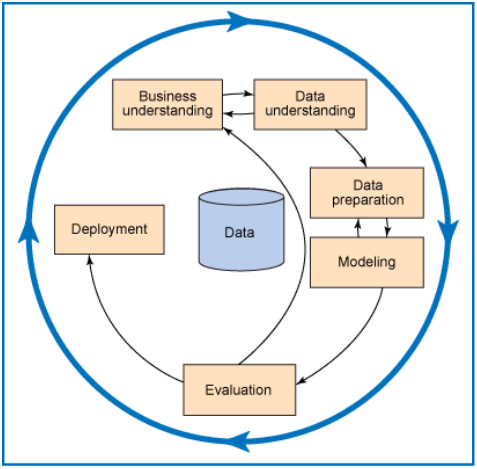
\includegraphics[width=0.7\textwidth]{figures/crispdm.png}
    \caption{Die 6 Phasen des CRISP-DM Modells}
    \label{fig:crispdm}
\end{figure}

Das Besondere an diesem Vorgehen ist, dass es an die teils nicht-lineare Struktur von KI- oder Deep-Learning-Projekten (vgl. Data Science Central, 2026) angepasst ist. Auch ein iteratives Vorgehen, welches in solchen Projekten angewendet wird, kann mit dem CRISP-DM-Modell abgebildet werden, wie auch in Abbildung \ref{fig:crispdm} zu sehen ist. Das ist wichtig, da die Schritte in der Praxis oft nicht linear abgearbeitet werden können und es wichtig ist, die Flexibilität zu haben, vorherige Schritte zu wiederholen, um deren Resultate zu verbessern oder anzupassen.

Um ein tieferes und besseres Verständnis für die sechs Phasen des CRISP-DM-Modells in der Theorie zu bekommen, werden diese im Folgenden kurz beschrieben. Im darauf folgenden Unterkapitel wird erläutert, wie diese Phasen in der Arbeit angewendet werden, um die Forschungsfrage zu beantworten.

\textbf{Business Understanding:} Bildet die Grundlage des Projekts und fokussiert sich auf das Verständnis der Projektziele sowie die Anforderungen aus geschäftlicher Perspektive.

\textbf{Data Understanding:} Eine erste Datensammlung wird durchgeführt, um ein initiales Verständnis für die Daten zu bekommen. Im Fokus steht hier die Identifikation relevanter Datenquellen sowie die Sammlung und erste Analyse der Daten, um deren Qualität und Struktur zu bewerten.

\textbf{Data Preparation:} Aufbereitung der Daten und Vorbereitung für die Modellierung. Die Phase umfasst die Bereinigung und Transformation der Daten in ein geeignetes Format sowie die Auswahl relevanter Features für die Modellierung.

\textbf{Modeling:} In dieser Phase werden verschiedene Modelle entwickelt und getestet, um die analytischen Ziele zu erreichen. Dies umfasst die Auswahl geeigneter Modellierungstechniken, die Entwicklung von Modellen und die Bewertung der Modelle hinsichtlich ihrer Leistung.

\textbf{Evaluation:} Hier werden die entwickelten Modelle bewertet und überprüft, ob sie die gestellten Anforderungen erfüllen. Die Phase umfasst die Überprüfung der Modellleistung sowie die Validierung der Modelle und die Entscheidung, ob das Modell in der Praxis eingesetzt werden kann.

\textbf{Deployment:} In der finalen Phase wird das entwickelte Modell in der Praxis verwendet. Hier wird das Modell implementiert, im Betrieb überwacht und bei Bedarf angepasst.